\documentclass[11pt]{beamer}
\usepackage[utf8]{inputenc}
\usepackage[T1]{fontenc}
%\usepackage{natbib}
\usetheme{Pittsburgh}
\usepackage{verbatim} 
\usepackage[english]{babel}
\usepackage{epstopdf}
\usepackage{multicol}%\columnseprule  0.4pt\raggedcolumns
%\titlegraphic{%\vspace*{1cm}
%	\includegraphics[width=2.5cm]{logo_udelar}
	%\hspace*{1cm}~%
%		\includegraphics[width=3.5cm]{logo_FCEA.png}
%}
\setbeamertemplate{navigation symbols}{}
\setbeamertemplate{footline}[frame number]
\AtBeginSection{ 
	\begin{frame}
		\frametitle{Index}
			\tableofcontents[currentsection]
	\end{frame}
}
\begin{document}
	\title{Modelos dinámicos y computacionales en Economía}
	\subtitle{Modelos Macroeconómicos Basados en Agentes}
	%\logo{}
	\institute{Licenciatura en Economía, FCEA, UDELAR}
	\date{21 de noviembre de 2023}

	%\subject{}
	%\setbeamercovered{transparent}
	%\setbeamertemplate{navigation symbols}{}
	\frame[plain]{
	\begin{figure}
	\centering
	\includegraphics[width=0.7\linewidth]{figuras/netlogo-title-wide-60}
	%		\caption{}
	\label{fig:netlogo-title-wide-60}
\end{figure}	
		\vspace{-1cm}
\maketitle
}
%\setbeamertemplate{background}{\includegraphics[width=2 cm]{logo_FCEA.png}}

\begin{frame}
\frametitle{Contenido de la clase:}
\begin{itemize}
	\item Macro ABM (MABM) en la literatura de ABM
	\item Características de los MABM
	\item Algunas clasificaciones
	\item Ejemplos
\end{itemize}
\end{frame}

\begin{frame}{Introducción}
\begin{quote}
\small    ``\textit{\textbf{When the crisis came, the serious limitations of existing economic and financial models immediately became apparent.}} Arbitrage broke down in many market segments, as markets froze and market participants were gripped by panic. \textit{\textbf{Macro models failed to predict the crisis and seemed incapable of explaining what was happening to the economy in a convincing manner.}} As a policy-maker during the crisis, \textit{\textbf{I found the available models of limited help.}} In fact, I would go further: \textit{\textbf{in the face of the crisis, we felt abandoned by conventional tools.}} In the absence of clear guidance from existing analytical frameworks, policy-makers had to place particular reliance on our experience. Judgement and experience inevitably played a key role.'' (Trichet\footnote{ Presidente del Banco Central Europeo durante el período 2003-2011}, 2010).
\end{quote}
\end{frame}


\begin{frame}{Introducción (cont.)}
\begin{quote}
    \small ``First, we have to think about how to characterise the homo
oeconomicus at the heart of any model. \textit{\textbf{The atomistic, optimising agents underlying existing models do not capture behaviour during a crisis period.}} We need to \textit{\textbf{deal better with heterogeneity across agents}} and the \textit{\textbf{interaction among those heterogeneous agents}}. We need to entertain \textit{\textbf{alternative motivations for economic choices}}. Behavioural economics draws on psychology to explain decisions made in crisis circumstances. \textit{\textbf{Agent-based modelling dispenses with the optimisation assumption and allows for more complex interactions between agents}}. Such approaches are \textit{\textbf{worthy of our attention}}.'' (Trichet, 2010)
\end{quote}    
\end{frame}

\begin{frame}
	\frametitle{MABM en la literatura de ABM} 
	\begin{itemize}
		\item \underline{Modelos Basados en Agentes (ABM):} modelos de sistemas adaptativos complejos donde una multitud objetos heterogéneos interactúan entre sí y con el ambiente.
		\item  \underline{Economía computacional basada en agentes (ACE):} ``El estudio computacional de los procesos económicos modelados como sistemas dinámicos de agentes interactivos'' (Tesfatsion, 2006)
		\item  \underline{ABM financieros:} modelos basados en agentes de un ``mercado artificial'' (habitualmente, una bolsa de valores) en donde los inversores (agentes) usan una serie de heurísticas para formar expectativas.
	\end{itemize}
\end{frame}

\begin{frame}
	\frametitle{MABM en la literatura de ABM} 
	\framesubtitle{(cont.)}
	\begin{itemize}
		\item \underline{Macro ABM (MABM):} se concibe a la macroeconomía como un sistema adaptativo complejo donde una multitud de agentes heterogéneos interactúan entre sí y con el ambiente.
		\item La heterogeneidad proviene del nivel educativo, productividad, tamaño, nivel de endeudamiento, apalancamiento, ingresos, riqueza, etc.
		\item Las variables macroeconómicas se computan en un enfoque ``bottom-up''$\rightarrow$ se deducen los objetos macroscópicos y sus leyes de comportamiento a partir de una multitud de objetos elementales que interactúan a partir de reglas simples.
	\end{itemize}
\end{frame}

\begin{frame}{MABM en la literatura de ABM}
\framesubtitle{Fuente: Delli Gatti (2013)}
\begin{figure}
    \centering
    \includegraphics[width=0.9\linewidth]{plots01/image827.png}
%    \caption{Caption}
    \label{fig:my_label}
\end{figure}
    
\end{frame}


\begin{frame}
	\frametitle{MABM en la literatura de ABM}
	\framesubtitle{Cómo realizar MABM?}
\begin{enumerate}
    \item Inicio: considerar una población de agentes heterogéneos (hogares, firmas, bancos, etc...)
    \item Teoría: describir una serie de reglas de comportamiento en el sistema (demanda y oferta de bienes, mano de obra, crédito, etc...)
    \item Codificación: trasladar estas reglas a líneas de código.
    \item Validación: 
    \begin{itemize}
        \item calibrar los parámetros
        \item correr las simulaciones
        \item analizar las propiedades emergentes de los datos simulados, tanto en forma \textit{cross-section} como las series temporales de las variables agregadas macroeconómicas.
        \item comparar estas propiedades con los ``hechos estilizados''.
    \end{itemize}
    
\end{enumerate}
\end{frame}

\begin{frame}
	\frametitle{Características de los MABM}
	\framesubtitle{Procesos autocatalíticos: procesos dinámicos con feedbacks positivos}
\begin{itemize}
    \item Esta característica asegura que el comportamiento de todo el sistema es dominado por la mayor tasa de crecimiento auto-catalítica en vez del elemento medio o mediano.
    \item Como resultado, el mundo se encuentra controlado por los extremos en vez del promedio.
    \item Esta es la clave para entender la emergencia de distribuciones libres de escala a nivel agregado. La relevancia de este tipo de distribuciones en economía se encuentra fuertemente reconocida en la econofísica (Mantegna \& Stanley, 2000) y en macroeconomía (Gabaix, 2011).
\end{itemize}
\end{frame}

\begin{frame}
	\frametitle{Características de los MABM}
\framesubtitle{Políticas a analizar $\rightarrow$ diferente a la macro tradicional}
    \begin{itemize}
        \item Debido a los feedbacks positivos, los shocks individuales pueden tener consecuencias agregadas: depende si el agente es lo suficientemente ``grande'' o se encuentra lo suficientemente ``conectado'' $\rightarrow$ incluso bajo la ausencia de shocks agregados, shocks individuales pueden generar fluctuaciones en el sistema.
        \item Debido a la heterogeneidad, los shocks agregados pueden tener consecuencias individuales: un shock agregado afecta no sólo a la media sino también a la varianza y al resto de los momentos de la distribución.
        \begin{itemize}
            \item un mismo shock agregado puede tener diferentes consecuencias según la distribución de respuestas de los agentes.
        \end{itemize}
        \item Las reglas de comportamiento pueden o no estar basadas en la optimización. 
        \item No se requieren condiciones de equilibrio.
    \end{itemize}
\end{frame}



\begin{frame}{Algunas clasificaciones}
    \begin{itemize}
        \item Ashraf, Gershman, Howitt (AGH)
        \item Complex Adaptive Trivial systems (CATS) $\rightarrow$ Delli Gatti, Gallegati, etc.
        \item Eurace@Unibi (EUBI) $\rightarrow$ Dawid, etc.
        \item Eurace en Genoa (EUGE) $\rightarrow$ Cincotti, Raberto, etc.
        \item Schumpeter meeting Keynes (K+S) $\rightarrow$ Dosi, Fagiolo, etc.
        \item JAMEL $\rightarrow$ Seppecher, Salle.
        \item Lagom $\rightarrow$ Jager, Mandel, etc.
    \end{itemize}
\end{frame}

\begin{frame}{Algunas clasificaciones}
    \framesubtitle{Schumpeter + Keynes}
    \begin{itemize}
        \item Objetivo: estudiar crecimiento y ciclos económicos.
        \item Número de agentes: > 500
        \item Número de parámetros: > 30
        \item Escala temporal: trimestres
    \end{itemize}
    \begin{figure}
        \centering
        \includegraphics[width=0.65\linewidth]{plots01/image918.png}
     %   \caption{Caption}
        \label{fig:my_label}
    \end{figure}
\end{frame}


\begin{frame}{Algunas clasificaciones}
    \framesubtitle{EURACE@UniBi}
   \begin{itemize}
        \item Objetivo: estudiar ciclos económicos de la economía europea, con estructura espacial.
        \item Número de agentes: > 1600
        \item Número de parámetros: > 50
        \item Escala temporal: días / meses
    \end{itemize}
    \begin{figure}
        \centering
        \includegraphics[width=0.70\linewidth]{plots01/image1009.png}
     %   \caption{Caption}
        \label{fig:my_label}
    \end{figure}
\end{frame}

\begin{frame}{Algunas clasificaciones}
    \framesubtitle{EURACE Genoa}
   \begin{itemize}
        \item Objetivo: estudiar la transición hacia una economía ``verde''.
        \item Número de agentes: > 600
        \item Número de parámetros: > 40
        \item Escala temporal: años
    \end{itemize}
    \begin{figure}
        \centering
        \includegraphics[width=0.45\linewidth]{plots01/image1100.png}
     %   \caption{Caption}
        \label{fig:my_label}
    \end{figure}
\end{frame}


\begin{frame}{Ejemplo de MABM}
\framesubtitle{Macroeconomics from the Bottom-up}
    \begin{figure}
        \centering
        \includegraphics[width=0.8\linewidth]{Captura desde 2022-09-24 22-12-12.png}
  %      \caption{Caption}
        \label{fig:my_label}
    \end{figure}
    \begin{multicols}{2}
\begin{itemize}
    \item \textbf{Agentes:} firmas, trabajadores (también como consumidores y hogares) y Bancos.
\item \textbf{Variables de estado:} Productividad, ganancias, salarios y deudas.
\item \textbf{Ambiente:} mercados:
\begin{itemize}
    \item de bienes.
\item de trabajo
\item de créditos
\end{itemize}
\end{itemize}        
    \end{multicols}
\end{frame}

\begin{frame}{Examples of MABM}
\framesubtitle{Macroeconomics from the Bottom-up}
Secuencia de eventos:
\begin{enumerate}
\item Las empresas calculan la producción basándose en la demanda esperada.
\item Se abre un mercado laboral descentralizado.
\item Se abre un mercado de crédito descentralizado.
\item Las empresas producen.
\item Se abre el mercado de bienes.
\item Las empresas pagarán préstamos y dividendos.
\item Las empresas y bancos sobrevivirán o morirán.
\item Reemplazo de empresas/bancos en bancarrota.
    \end{enumerate}
\end{frame}


\begin{frame}{Ejemplo de MABM}
\framesubtitle{Agentes heterogéneos y redes de créditos\footnote{Riccetti, L., Russo, A., \& Gallegati, M. (2013). Leveraged network-based financial accelerator. \textit{Journal of Economic Dynamics and Control, 37}(8), 1626-1640.}}
\begin{itemize}
    \item Este modelo, que se encuentra en Bargigli et al. (2016)\footnote{Bargigli, L., Caiani, A., Riccetti, L., \& Russo, A. (2016). A Simple Model of Business Fluctuations with Heterogeneous Interacting Agents and Credit Networks. In \textit{Economics with Heterogeneous Interacting Agents} (pp. 29-102). Springer, Cham.}, busca reproducir cómo los ciclos económicos se ven alterados por mecanismos que se refuerzan a sí mismos.
    \item Idea principal: un shock en el resultado de las empresas las hace menos propensas a invertir. A su vez esto genera una caída en los resultados, por lo cual se genera un círculo vicioso.
\end{itemize}
\end{frame}

\begin{frame}{Ejemplo de MABM}
\framesubtitle{Agentes heterogéneos y redes de créditos (cont.)}
\begin{itemize}
    \item Feedback positivo: aumentado por factores financieros $\rightarrow$  ``acelerador de apalancamiento'' (Riccetti et al., 2013)
    \begin{itemize}
        \item el shock negativo hace que los bancos presten menos a las empresas.
        \item restricciones en el crédito a las empresas: menor cantidad de créditos o mayores tasas de interés
        \item esto fuerza a las empresas a un menor apalancamiento, así como a una menor inversión y menores resultados.
    \end{itemize}
    \item importante: una crisis que comienza en el sector financiero puede generar una recesión en el sector real de la economía.
\end{itemize}
\end{frame}

\begin{frame}{Ejemplo de MABM}
\framesubtitle{Agentes heterogéneos y redes de créditos (cont.)}
\begin{itemize}
    \item Acelerador financiero basado en la estructura de interrelaciones de la economía: ``network-based''.
    \begin{itemize}
        \item Existe una red de créditos en la economía que puede producir una avalancha de quiebras.
        \item La quiebra de una empresa genera problemas para los bancos, por las deudas incobrables. 
        \item Si los bancos quiebran, se generan distorsiones en el mercado de créditos de la economía.
        \item Si los bancos llegan a sobrevivir, reaccionan restringiendo el crédito o aumentando la tasa de interés.
    \end{itemize}
    \item Feedback: Sector no financiero $\rightarrow$ sector financiero $\rightarrow$ sector no financiero.
\end{itemize}
\end{frame}

\begin{frame}{Ejemplo de MABM}
\framesubtitle{Agentes heterogéneos y redes de créditos (cont.)}
Orden del modelo en R:
\begin{multicols*}{2}
\begin{enumerate}
\scriptsize
    \item Bancos calculan su tasa de interés específica $R_{b,t}$
    \item Mecanismo de asignación en el mercado de créditos $link_{f,b}$
    \item Firmas actualizan su nivel de leverage $leverage_{i,t}$
    \item Firmas calculan su demanda de créditos $B_{i,t}$
    \item firmas calculan su capital financiero $K_{i,t}$
    \item Firmas calculan su producción objetivo $Y_{i,t}$
    \item Firmas actualizan el precio $p_{i,t}$
    \item Firmas calculan su tasa de interés específica $R_{i,t}$
    \item Firmas calculan beneficios $Pr_{i,t}$
    \item Firmas calculan el nivel de riqueza $A_{i,t}$ y observan si están en default o no $fall_{i,t}=f(A_{i,t})$
    \item Firmas calculan el ratio de pérdidas (si la empresa quiebra) $LGD_{i,t}=f(A_{i,t},B_{i,t})$ 
    \item Bancos calculan depósitos $D_{b,t}$
    \item Bancos calculan ``deuda incobrable'' $bad_{b,t}$
    \item Bancos calculan beneficios $Pr_{b,t}$
    \item Bancos actualizan sus beneficios netos y chequean si quiebran o no $fall_{b,t}=f(A_{b,t})$
\end{enumerate}
\end{multicols*}
\end{frame}


\begin{frame}{Ejemplo de MABM}
\framesubtitle{Agentes heterogéneos y redes de créditos (cont.)}
\begin{itemize}
    \item Función de producción de las empresas
\begin{equation*}
    Y_{i,t}=\phi K^{\beta}_{i,t}
\end{equation*}
\item Nivel de endeudamiento
\begin{equation*}
    B_{i,t}=A_{i,t} leverage_{i,t}
\end{equation*}
\item Precio esperado:
\begin{equation*}
    p^{e}_{i,t+1}=p_{i,t}
\end{equation*}
\item Apalancamiento: depende de la tasa de interés esperada y del retorno de la inversión
\item Heterogeneidad: determinada por su tamaño, su riqueza y por su objetivo de apalancamiento.
\end{itemize}
\end{frame}

\begin{frame}{Ejemplo de MABM}
\framesubtitle{Agentes heterogéneos y redes de créditos (cont.)}
\begin{itemize}
    \item Regla de tasa de interés de los Bancos: depende de la tasa de interés del Banco Central, del Banco y del componente de riesgo de la empresa.
    \item Elección de Banco: siguiendo una regla de ``strategic link formation''. El Banco se cambia con una probabilidad que depende de la diferencia entre tasas de interés.
    \item Beneficios de las empresas:
    \begin{equation*}
        Pr_{i,t}=p_{i,t}Y_{i,t}-R_{z,i,t}B_{i,t}
    \end{equation*}
    \item Patrimonio de las empresas:
    \begin{equation*}
        A_{i,t+1}=A_{i,t}+Pr_{i,t} \rightarrow \text{ si $A_{i,t+1}<0$, bancarrota}
    \end{equation*}
\end{itemize}
\end{frame}

\begin{frame}{Ejemplo de MABM}
\framesubtitle{Agentes heterogéneos y redes de créditos (cont.)}
\begin{itemize}
    \item Como la cantidad de empresas se mantiene fija, se crea una nueva empresa, con bajo capital.
    \item En caso de quiebra de una empresa, el Banco prestador sufre una pérdida:
    \begin{equation*}
        LGD_{i,t}=\dfrac{-(A_{i,t}+Pr_{i,t})}{B_{i,t}}
    \end{equation*}
    \item Patrimonio de los Bancos:
    \begin{equation*}
        A_{z,t+1}=A_{z,t}+Pr_{z,t} \rightarrow \text{ si $A_{z,t+1}<0$, bancarrota}
    \end{equation*}
\end{itemize}
\end{frame}

\begin{frame}{Ejemplo de MABM}
    \framesubtitle{Nota complementaria: cómo comunicamos los modelos?}
	Por qué debemos \underline{documentar} adecuadamente los ABM en las Ciencias sociales?
	\begin{itemize}
		\small		\item \textit{``Lack of a common methodological standard on how to build, describe, analyze, evaluate and replicate ABM''} (Squazzoni, 2010).
		\item \textit{``..the greater freedom they have granted to researchers (in terms of model design) has often degenerated in a sort of anarchy (in terms of design, analysis and presentation)''} (Ricchiardi et al., 2006).
		\item \textit{``...a primary obstacle is establishing a common language for effective communication among researchers with diverse backgrounds''} (Garibay et al., 2019).
	\end{itemize}
\end{frame}

\begin{frame}{Ejemplo de MABM}
    \framesubtitle{Nota complementaria: cómo comunicamos los modelos?}
	Qué es el \underline{ODD Protocol}?
	\begin{itemize}
		\item Acrónimo de \textbf{O}verview, \textbf{D}esign concept and \textbf{D}etails.
		\item Desarrollado por Grimm et al. (2006).
		\item Propósito (Grimm et al, 2013): 
		\begin{itemize}
			\item Facilitar la escritura y lectura de descripciones de modelos, haciéndolas comprensibles y completas.
\item Permitir la replicación de los modelos basados en agentes (ABM).
\item Establecer un conjunto de conceptos de diseño que deben tenerse en cuenta al desarrollar un ABM.
\item Se pretende describir adecuadamente los aspectos esenciales de los modelos.
\end{itemize} 
		\item \textit{``create a generic format and a standard structure by which all ABMs could be documented''} (Grimm et al., 2010)
	\end{itemize}
\end{frame}

\begin{frame}{Ejemplo de MABM}
    \framesubtitle{Nota complementaria: cómo comunicamos los modelos?}
	\begin{figure}
		\centering
		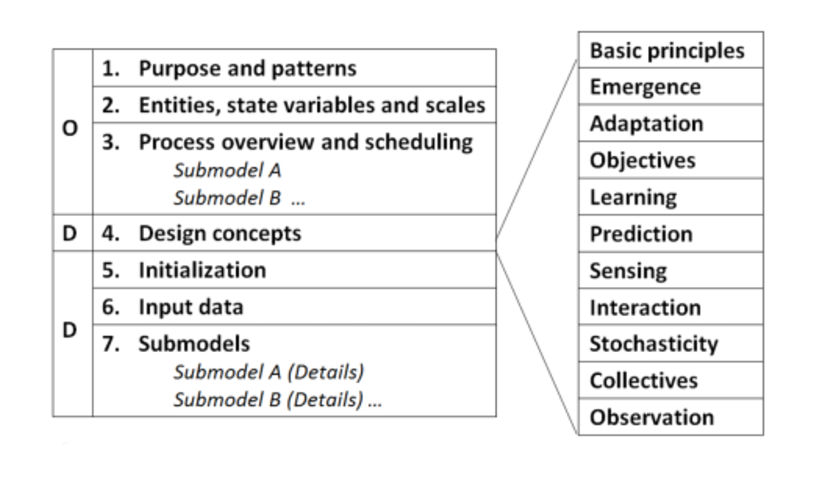
\includegraphics[width=0.7\linewidth]{ODD_structure}
		\caption{Estructura del modelo, siguiendo el Protocolo ODD. (Grimm et al., 2020.)}
		\label{fig:oddstructure}
	\end{figure}
\end{frame}

\begin{frame}{Ejemplo de MABM}
    \framesubtitle{Nota complementaria: cómo comunicamos los modelos?}
\begin{figure}
    \centering
    \includegraphics[width=\linewidth]{Captura desde 2022-09-27 11-45-27.png}
 \small   \caption{Simulación de ``Macroeconomics from the bottom-up'', en NetLogo}
    \label{fig:my_label}
\end{figure}
Descripción y modelo en NetLogo de ``Macroeconomics from the Bottom-up'' (Delli Gatti et al., 2011):
\url{https://github.com/alexplatasl/BAMmodel}
    
\end{frame}

\end{document}
